% $Id: adjustment.tex 9292 2021-08-01 03:27:38Z mskala $

%
% MSK 007 adjustment procedure
% Copyright (C) 2017  Matthew Skala
%
% This program is free software: you can redistribute it and/or modify
% it under the terms of the GNU General Public License as published by
% the Free Software Foundation, version 3.
%
% This program is distributed in the hope that it will be useful,
% but WITHOUT ANY WARRANTY; without even the implied warranty of
% MERCHANTABILITY or FITNESS FOR A PARTICULAR PURPOSE.  See the
% GNU General Public License for more details.
%
% You should have received a copy of the GNU General Public License
% along with this program.  If not, see <http://www.gnu.org/licenses/>.
%
% Matthew Skala
% https://northcoastsynthesis.com/
% mskala@northcoastsynthesis.com
%

\chapter{Adjustment}

A properly built module will probably sound okay if you skip some or all of
these final adjustment steps (for instance, because of not having the right
test equipment), but to really operate at its intended level of performance,
the module should be adjusted carefully to compensate for the natural
variations in the components.

Do the pre-adjustment in the previous chapter on Board~3 first.

For the steps in this chapter, you will need (in addition to specific items
mentioned in the individual steps) a multimeter, a tool such as a small
screwdriver for adjusting trimmers, a Eurorack power supply, and your
complete, fully assembled, MSK~007 Leapfrog Filter module.

\section{Short-circuit test}

Without power applied to the module, check for shorts between the three
power connections on the Board~3 Eurorack power connector, testing each pair
in both directions (six tests in all).

\noindent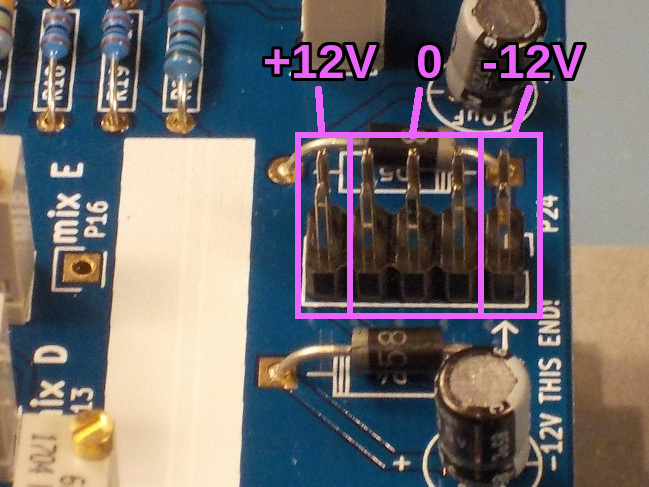
\includegraphics[width=\linewidth]{power-pinout.jpg}

Ideally, you should use an ohmmeter's
``diode test'' range for this, and it should read infinite in the reverse
direction (positive lead to $-$12V and negative lead to each of the other
two, as well as positive lead to ground and negative to $+$12V) and greater
than 1V in the forward direction (reverse those three tests).  If any of
these six measurements is less than 1k$\Omega$ or 1V, then something is
wrong with the build and you should troubleshoot it before applying power.

Plug the module into a Eurorack power supply and make sure
neither it nor the power supply emits smoke, overheats, makes any unusual
noises, or smells bad.  If any of those things happen, turn off the power
immediately, and troubleshoot the problem before proceeding.

\emph{Optional}: Plug the module into a Eurorack power supply
\emph{backwards}, see that nothing bad happens, and congratulate yourself on
having assembled the reverse-connection protective circuit properly. 
Reconnect it right way round before proceeding to the next step.

\section{DC offsets}

For this step you will need the capability to measure DC voltages, including
the DC component of an audio-rate signal.  If you are using a voltmeter,
make sure it will not be confused by a signal that includes both AC and DC. 
If you are using an oscilloscope, make sure it is set to DC-coupled input.

The MSK~007 is a DC-coupled filter and in principle, DC applied to the input
can pass all the way through to the output.  That can be advantageous in
some patches where you may want to pass a control voltage or envelope
through the filter.  However, it has the disadvantage that offsets created
by the normal tolerances of the amplifier chips can add up (especially
around the multiple feedback loops).

Including a trimmer for every possible offset-introducing component would be
prohibitively expensive and complicated.  Instead, the MSK~007 has two: R50
on Board~3, which trims offset in the filter core, and R89 on Board~1, which
trims offset in the VCA circuit.  The following adjustment procedure is a
trade-off intended to reduce offset as much as possible under common
operating conditions.  Some DC offset will still remain at the edges of the
normal operating range (for instance, very high or low cut-off frequencies).

Disconnect all cables from the filter.  Apply power.  Set coarse and fine
tuning to their midpoints, exponential and linear FM to zero, VCA mode to
feedback (toggle switch left), and VCA amount to minimum.

You should have set R50 on Board~3 and R89 on Board~1 to their midpoints
before installing them (or R50 during pre-adjustment), but if not: measure
the voltage at P14 ``DC'' (on Board~3 near R50) and adjust R50 to bring this
voltage to zero; and measure the voltage at P19 (on the upper edge of
Board~1 near R89) and adjust R89 to bring this voltage to zero.

Measure the output voltage of the module, either by plugging into the output
jack or at P11 on the bottom edge of Board~1 (which is directly connected to
the output jack).  It should be a pure DC voltage.  Adjust R50 on Board~3 to
bring this voltage to zero.

Turn the VCA amount knob up to maximum.  The module should start to
oscillate, probably at a frequency of about 200Hz (wide tolerance on
frequency) and with voltage at least 4V peak to peak.  Measure the \emph{DC
offset} of the AC output voltage and adjust R89 on Board~1 to bring the
offset to zero.

Switch the VCA mode to output (toggle switch right) and measure the DC
output voltage.  Adjust it with R89 on Board~1 \emph{halfway} from wherever
it currently is, to zero.

\section{Optional: integrator phase shifts}

If you did the pre-adjustment carefully, your module will probably already
give something very close to the designed response curve.  One significant
advantage of the leapfrog topology is that it is especially tolerant to
inaccuracies in component values: the curve will not change much with small
misadjustments.  However, the pre-adjustment procedure only takes into
account the tolerance variation of the components on Board~3.  There are
some components on Board~2 (particularly the integration capacitors and the
control current distribution system) which also affect filter performance,
and so to really adjust everything as well as possible, it is necessary to
do a final adjustment of five integrator phase shifts on the fully
assembled module.

In my experiments on prototype modules, doing the full adjustment procedure
seems to provide a very small improvement in stopband attenuation, but makes
very little difference to the main filter curve.  And the phase shift
adjustment has the disadvantage of being time-consuming and annoying.  The
five trimmers all mutually interact and the phase shifts one must measure to
get them set right, are not easy to measure accurately.  There is the danger
that if you do it and screw it up, you may end up with a worse filter than
if you had just stopped at the pre-adjustment.  So for do-it-yourselfers I
am describing this procedure as ``optional.'' You can do it if you want to;
in theory, it makes things better; but it is quite likely that you won't be
able to hear or even measure a difference between doing it and not doing it. 
If you do mess things up with a bad full-adjustment procedure, it is not a
big problem.  You can always separate Board~3 from the rest of the module
and re-do the pre-adjustment alone to go back to that level of performance.

For this step you will need the capability to tune the module to
self-oscillation at 740Hz or the F$\sharp$ one and a half octaves above
middle C (either by measuring its output frequency directly, or by tuning to
zero-beat against a known source of this frequency); to generate a clean
sine wave at this same frequency; and to measure the phase or timing
difference between two such sine waves.  A two-trace digital oscilloscope
will probably do most of the measuring functions conveniently, and a
computer can act as a signal generator.  Alternatively, a modular
synthesizer VCO with a sine output will work as the signal generator if you
have some way to tune it, and a dual-trace analog oscilloscope can be used
for the phase measurements with some care.  It may also be possible to use
software on a computer, with the two signals fed in as left and right stereo
channels to the audio interface, to do the phase measurements.  Details of
how to use different kinds of test equipment are not covered here; this
description just gives the needed adjustment targets assuming you know how
to use your equipment.

Disconnect any input or modulation signals and apply power to the filter. 
Set coarse and fine tuning to their midpoints, exponential and linear FM to
zero, VCA mode to feedback, and VCA amount to maximum.  Monitor the output;
the module should produce a sine wave in the range of a few hundred Hz.

Tune the module with the coarse and fine tuning, and reduce the VCA amount,
until it oscillates at the F$\sharp$ one and a half octaves above middle C
(12-EDO concert pitch); that is theoretically 739.9888Hz, but it is probably
best to aim for exactly 740Hz.  Measure the frequency with the VCA amount
just high enough to keep the oscillation stable.  \emph{From this point on,
to the end of the phase-shift adjustment, don't touch the tuning knobs.}

Note that it may be difficult to make some of these adjustments precisely. 
I give the target values down to hundredths of a degree of phase, but
(especially for the phase shifts on integrators B and A, the last ones to be
adjusted, which seem especially finicky) it may not be possible to really
adjust them within better than one or two whole degrees.  Just do the best
you can.  The closer these adjustments are to perfection, the better the
module will comply with its theoretical response curve; but even significant
errors in the adjustment will only degrade performance a little bit.

Note that there will be moderate differences in amplitude (up to a factor of
two in voltage) among the signals measured in the next few steps, and some
may have noticeable DC offsets.  That is normal; the important differences
to measure are in their phases.  However, be on the lookout for clipping
indicated by flat tops or bottoms on the waveforms.  If you see that,
your input reference waveform level is too high and it may be rendering the
measurements inaccurate.  Turn it down.

Turn the VCA amount down to zero.  The module will stop oscillating; but
leave the VCA mode switch set to feedback mode.  Feed a pure sine wave of
the same reference frequency, 739.9888Hz or 740Hz, into the input,
preferably with an amplitude of about 5V peak to peak.  I use a Hikari Sine
oscillator patched through an attenuator.

In the following steps, be careful to adjust the right trimmers.  The phase
measurements are taken at test points near the centre of the board, labelled
``mix~A,'' ``mix~B,'' and so on; but the trimmers to adjust are the time
constant trimmers, nearer the edges and labelled ``TC~A,'' ``TC~B,'' and so
on, not the mix trimmers nearest the test points.  The mix trimmers were set
in the pre-adjustment step and if you change them, you will need to separate
the boards again to take the necessary measurements for returning them to
the correct positions.  Throughout the phase shift adjustments, if adjusting
a trimmer seems to have no effect on the measurement you are taking,
\emph{stop} and make sure you are turning the correct trimmer.  Some of them
are more sensitive than others, but every one should make some measureable
difference.

If during the following steps you find there is not enough adjustment range
on a trimmer to hit the desired measurement, then leave it at the end of its
range nearest the desired setting, and if necessary go around the six
adjustments steps again until you come back to it.  The interactions between
the adjustments mean that on the next visit it will probably not be pushed
to an extreme.  If that doesn't seem to work, it may be necessary to re-tune
the module to oscillate at the reference frequency, and then try again.  If
even \emph{that} doesn't allow the trimmers to be adjusted to their desired
settings, then there may be a build error and you should troubleshoot for
things like solder bridges.

Measure the phase difference between the signals at P16, labelled ``mix~E''
on the back of the module, and P13, labelled ``mix~D.''  Adjust R27,
labelled ``TC~E,'' so that the P16 ``mix~E'' signal leads the P13 ``mix~D''
signal by 45.59$^\circ$ or 171.15$\mu$s; your equipment may
instead display this as a lag of 314.40$^\circ$ or 1180.19$\mu$s.

Measure the phase difference between the signals at P13, labelled ``mix~D''
on the back of the module, and P10, labelled ``mix~C.''  Adjust R26,
labelled ``TC~D,'' so that the P13 ``mix~D'' signal leads the P10 ``mix~C''
signal by 40.98$^\circ$ or 153.84$\mu$s; your equipment may
instead display this as a lag of 319.02$^\circ$ or 1197.54$\mu$s.

Measure the phase difference between the signals at P10, labelled ``mix~C''
on the back of the module, and P9, labelled ``mix~B.''  Adjust R9,
labelled ``TC~C,'' so that the P10 ``mix~C'' signal leads the P9 ``mix~B''
signal by 30.36$^\circ$ or 113.96$\mu$s; your equipment may
instead display this as a lag of 329.64$^\circ$ or 1237.40$\mu$s.

Measure the phase difference between the signals at P9, labelled ``mix~B''
on the back of the module, and P8, labelled ``mix~A.''  Adjust R8,
labelled ``TC~B,'' so that the P9 ``mix~B'' signal leads the P8 ``mix~A''
signal by 48.68$^\circ$ or 182.75$\mu$s; your equipment may
instead display this as a lag of 311.32$^\circ$ or 1168.63$\mu$s.

Measure the phase difference between the signals at P8, labelled ``mix~A''
on the back of the module, and P7, labelled ``mix~IN.''  Adjust R7,
labelled ``TC~A,'' so that the P8 ``mix~A'' signal leads the P7 ``mix~IN''
signal by 14.40$^\circ$ or 54.04$\mu$s; your equipment may
instead display this as a lag of 345.60$^\circ$ or 1297.31$\mu$s.

Repeat the above steps a second time, starting from the measurement of the
lag between P16 ``mix~E'' and P13 ``mix~D.''

These measurements are summarized in Table~\ref{tab:adjust-targets}.

\begin{table}
\begin{tabular}{c|lD{.}{.}{3}D{.}{.}{3}}
  trimmer & \multicolumn{1}{c}{measure} & \multicolumn{2}{c}{target} \\ \hline
  TC~E\bigstrut[t] & MIX~E--MIX~D & 45.59^\circ & 314.40^\circ \\
  TC~D & MIX~D--MIX~C & 40.98^\circ & 319.02^\circ \\
  TC~C & MIX~C--MIX~B & 30.36^\circ & 329.64^\circ \\
  TC~B & MIX~B--MIX~A & 48.68^\circ & 311.32^\circ \\
  TC~A & MIX~A--MIX~IN & 14.40^\circ & 345.60^\circ \\
\end{tabular}
\caption{Measurement targets for time constant
adjustment}\label{tab:adjust-targets}
\end{table}

Optional cross-checks:  Measure the phase difference between the module
input and module output.  They should be close to 180$^\circ$ apart. 
Disconnect the input and turn the VCA amount back up until the module
oscillates.  It should still be close to 740Hz.  There is no specific
guidance on \emph{how} close these measurements should be to their targets.

\section{Tracking (with automated test)}

``Tracking'' refers to the slope of the V/octave control voltage response. 
It should be exactly 1.0V/octave.  The trimmer R77, located on Board~1,
adjusts this response.

The best way to adjust this setting, if you have the equipment and
skills, is by hooking up the module to a computer that can send it control
voltages, measure the output frequency in self-oscillation, and compute an
estimate of the current V/octave ratio, which allows realtime feedback as
you adjust the trimmer.  I provide a piece of software in the file
\texttt{voct-0.1.tar.gz} to support this process.

The software is written for the Linux ALSA MIDI and PCM drivers, and it
includes hardcoded assumptions about things like device numbers.  \emph{You
need C programming skills to use this software.  I will not provide
support on it.}  If you cannot modify the software as needed to suit your
installation, then I recommend using the manual tracking procedure in the
next section instead.

Read the C source code and make any appropriate changes for your
installation.  Compile it.  Connect your MIDI-to-CV interface to the V/oct
input on the MSK~007, and connect the MSK~007's audio output to your
computer's audio input.  Remove any other cables from the MSK~007, set the
VCS mode to feedback, the VCA amount high enough for reliable oscillation,
and exponential and linear FM to zero.  Optionally (requires other
appropriate software, not included), send MIDI note 69 to the MIDI interface
and adjust the tuning of the MSK~007 to make it oscillate at 440Hz;
otherwise set the coarse tuning to about 10 o'clock and the fine to its
midpoint. 
Adjut the sensitivity of the audio input to bring the Leapfrog's signal to
about 50\%\ of full scale.  Run the \texttt{vcoslope} software.

The vcoslope program sends random MIDI notes, makes brief recordings of the
oscillator output, and attempts to fit an exponential function (using linear
regression) to the note/frequency data in the last $N$ notes, for several
different values of $N$.  From that it can determine the current sensitivity
of the V/octave input.  Using multiple frequencies to test like this gives
better accuracy than would be the attainable with just testing at two
frequencies (as in the standard manual procedure).  Using notes in random
order is preferable to testing them in an increasing or decreasing sequence,
because of self-heating effects in the exponential converter.  The program
tries multiple sample sizes (the most recent 10, 32, 100, and 316 points)
to allow both quick feedback on any trim changes, and accurate results over
longer periods.

It will start producing lines of output, one every few seconds.  Each
line starts with a decimal sequence number (1, 2, 3, \ldots) and the MIDI
note number that was sent.  The next two columns are the measured frequency
in Hertz, and the number of octaves plus or minus that is relative to the
440Hz reference pitch.  Then come up to four columns of V/octave estimates:
the first determined from the last 10 notes tested, the second from the last
32 notes, then 100 notes, then 316 notes.  These columns each show up only
once there have been the requisite number of notes, so at first there will
be no such column, then the first one will appear on the tenth note, then
the second at note 32, and so on.

Let the program run for at least 10 or 20 notes so you can get some idea of
the module's current V/octave response.  Then try adjusting R77 one turn
clockwise.  Watch for another 10 lines of output.  The 10-note V/oct
estimate should start to move, then settle in on a new value.  From there
you should be able to estimate how far (how many turns) and in which
direction you need to adjust R77 to bring the response to 1.000V/oct.  Try
to do that.  As you get in closer, the natural noise in the V/oct numbers
may become significant in relation to the sizes of adjustment you are
making.  In that case, switch to one of the slower-updating columns to get a
more stable reading (larger sample size).  You will need to wait longer
between adjustments for those columns to reach full precision.  Continue
until you have the module performing as accurately as you want, or until you
run out of patience.

\section{Tracking (by hand)}

This simpler tracking procedure does not require computer skills, only the
ability to send reproducible control voltages of 0V and 1V to the filter and
test the resulting frequencies.  It is somewhat less accurate because it
tests only two frequencies instead of averaging over many, but it is similar
to the way people commonly adjust VCOs, which have much more demanding
accuracy requirements than most VCFs.

A North Coast Synthesis MSK~008 Octave Switch, assuming it has itself been
properly adjusted, makes an ideal voltage source for the following
procedure.

Hook up your control voltage source to the filter's V/oct input, set up your
equipment as necessary to test the frequency of the audio output, disconnect
any modulation signals, and power up the filter.  Set the VCA mode to
feedback, VCA amount to just enough to get a stable oscillation, and set
both modulation controls to zero.

Send a 0V control voltage to the filter.  Tune it with the coarse and fine
tuning knobs to an oscillation frequency of 440Hz (or any arbitrary
frequency of your choice, but this one is convenient).

\emph{Without changing the tuning knob settings,} send a 1V control voltage
to the filter.  Adjust R77, not the tuning knobs, to bring the oscillation
frequency to 880Hz (or twice the initial frequency if you are using
something other than 440Hz).

Send a 0V control voltage and test the output frequency; is it 440Hz or your
chosen other reference frequency?  If not, adjust the tuning knobs to make
it so.  Repeat these two steps, of alternately adjusting for the low
frequency with 0V and the tuning knobs, and the high frequency with 1V and
the trimmer potentiometer, until both readings are reliably what they should
be without seeming to need further adjustment.

For even better accuracy:  use two control voltages more than 1V apart, and
a correspondingly wider frequency range.  For instance, an MSK~008 octave
switch can conveniently
generate $+$1V and $-$1V, which could be used with reference frequencies of
880Hz and 220Hz to set tracking over two octaves instead of just one.
